% -*- latex -*-
In this section we will discuss the  \acf{IMP} model for parallel programming;
see~\cite{Eijkhout:ICCS2012,Eijkhout:hips2014}
for further details. Here we limit ourselves to the aspects of the model that
interact with hardware design.

\subsection{Brief introduction}

\ac{IMP} is a theoretical model for expressing parallel algorithms.
It operates on a high level of abstraction, but it requires the programmer
to specify enough about parallelism to make these concepts 
translatable to efficient code; see below for proof of this contention.

The \ac{IMP} model
is based on distributions of data and work. Unlike many other programming systems,
\ac{IMP} has distributions as first-class objects and provides an algebra
of operations on and transformations between distributions. Thus,
\textbf{IMP translates to an intermediate representation 
expressed in a rich vocabulary of data motion concepts}.
The \ac{IMP} model is flexible enough
to handle traditional Cartesian structures, but also sparse data
and even distributions with redundant duplication. (That latter option
means that resilience is formally expressible in \ac{IMP} through
manipulating the distribution mechanism.)

The theory behind \ac{IMP} derives data dependencies 
through formal transformations between distributions.
Specifically, each parallel operations (a~`kernel')
is based on the distributions on the input and output objects,
as well as a distribution that is defined by the structure
of the calculation. Reconciling these three distributions
gives tasks and task data dependencies as formally 
derived objects.

Since \ac{IMP} is based on formal reasoning, it is not dependent on
any parallelism model, and in fact it can be shown to generalize both
distributed memory message passing and shared memory task models.  
We summarize this workflow in figure~\ref{fig:imp-structure}.
\begin{figure}[ht]
  \includegraphics[scale=.14]{graphics/imp_structure}
  \caption{Block diagram of programming with IMP}
  \label{fig:imp-structure}
\end{figure}
As
a proof-of-concept of the IMP framework we implemented a simple example, the
one-dimensional heat equation, as a C++ class library along the \ac{IMP} formalism, and
compiled it twice, once as MPI code, and once using OpenMP
tasks~\cite{Eijkhout:hips2014}.  We compared this code to manually
produced reference codes.
\begin{figure}[ht]
\leavevmode\hbox{%
  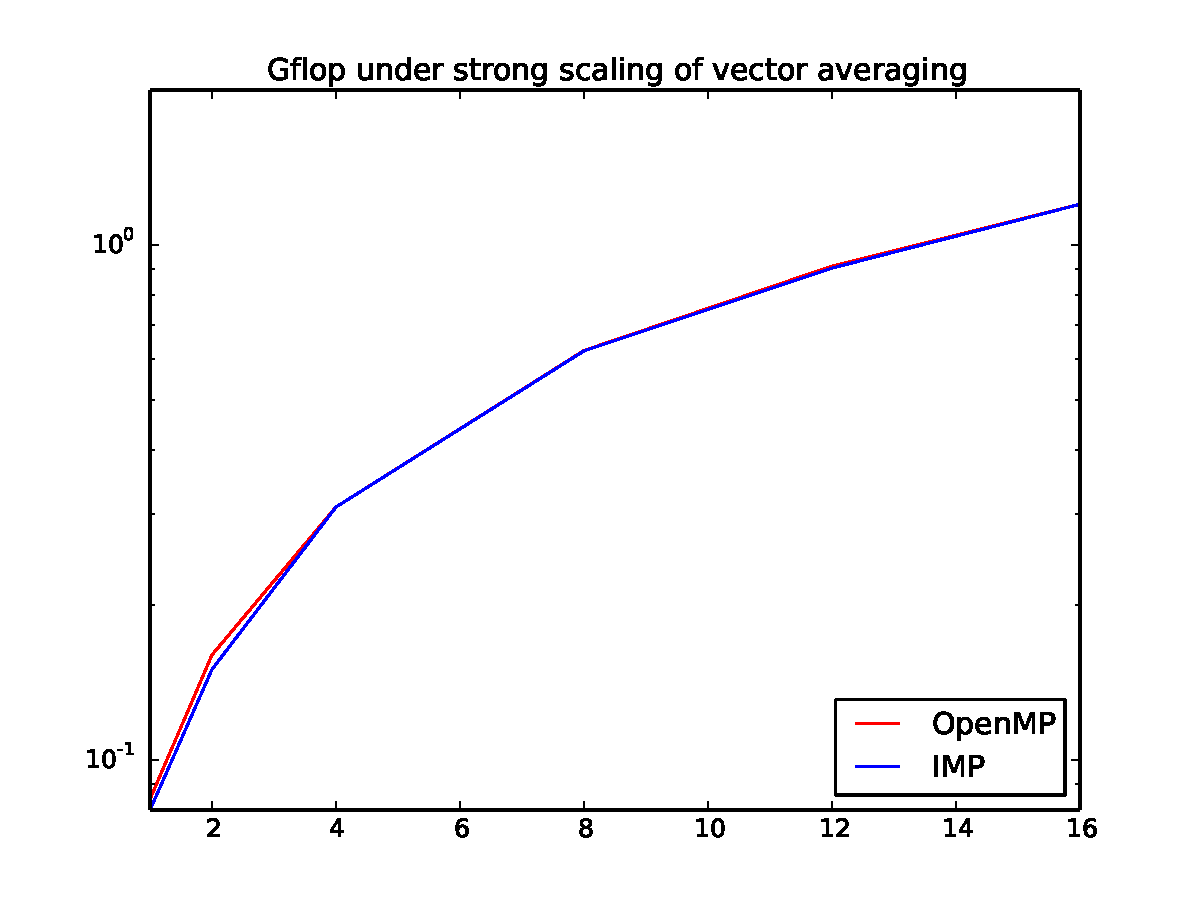
\includegraphics[scale=.4]{graphics/omp_scaling}
  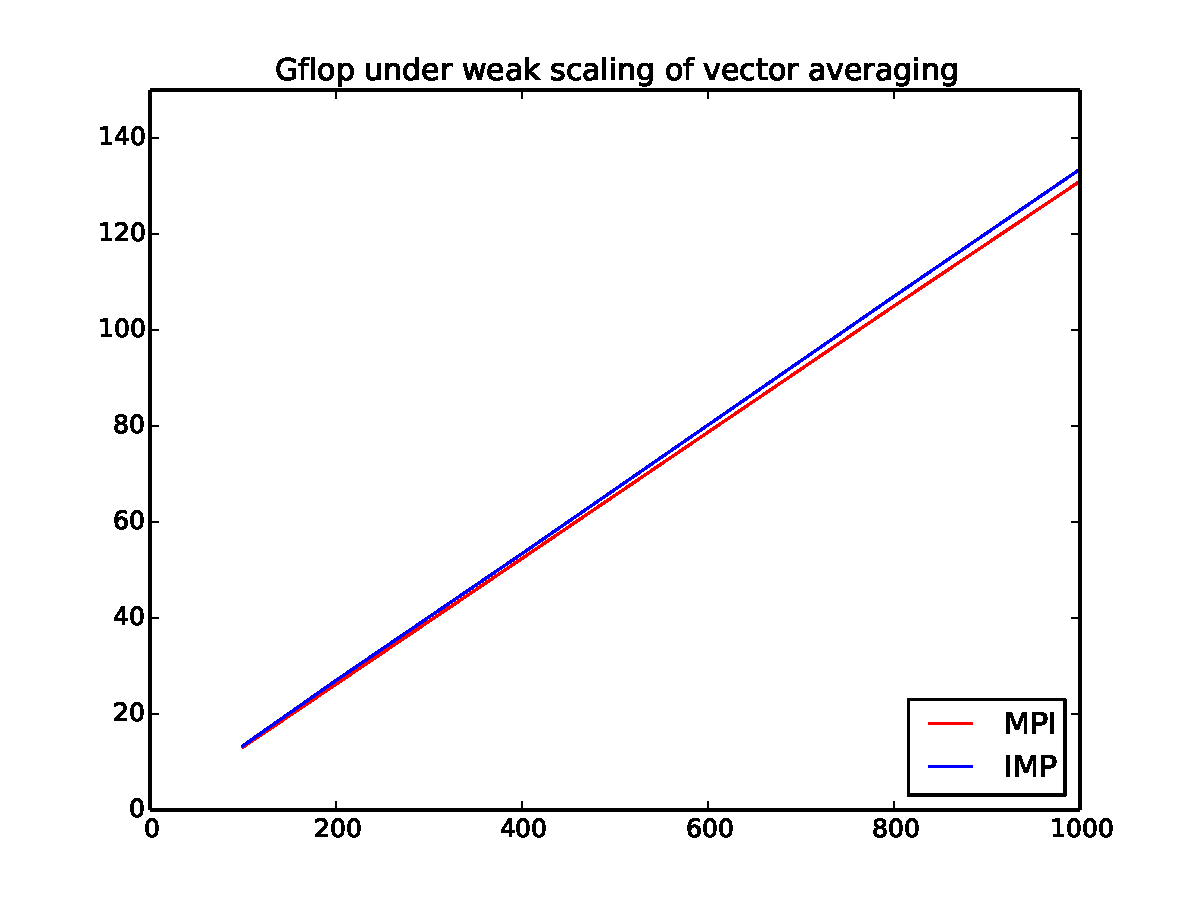
\includegraphics[scale=.4]{graphics/mpi_scaling}
  }
  \caption{Scaling behaviour of OpenMP and MPI realizations of the example IMP code,
  compared to manually produced reference codes.}
  \label{fig:scale}
\end{figure}
Figure~\ref{fig:scale} shows that both with OpenMP and MPI the 
performance behaviour,
possibly after startup phenomena,
is identical within 2--3\%.

While we target two parallel programming backends here,
the IMP model can as easily accomodate hybrid forms of parallelism.
In that case, IMP code would be realized as a mix of these backends,
and not using any PGAS system.

\subsection{IMP as a basis for co-design}

Above we reasoned that the poor performance on contemporary processors is due to 
deficient semantics of the processor/memory interface.
The \ac{IMP} model can remedy this, since it can formally derive
all data dependencies in a parallel algorithm.

\begin{wrapfigure}{r}{8cm}
%\begin{figure}[ht]
  \includegraphics[scale=.1]{graphics/dram-semantics}
  \caption{Illustration of different transfer demands on halo data
    for lexicographic stencil update}
  \label{fig:dram-halo}
%\end{figure}
\end{wrapfigure}
%
For instance, an \ac{IMP} analysis of an algorithm not only knows
what data is needed in a kernel, it also knows its structure
and when it is available. This means for instance:
\begin{itemize}
\item An \ac{IMP} kernel can provide semantic information on requested
  data to the DRAM controller, allowing it to schedule an efficient
  transfer. Possible DRAM semantics could include whether data is
  contiguous or strided, but also latency and bandwidth properties
  such as its anticipated absorption rate; see
  figure~\ref{fig:dram-halo}.
\item Rather than data being transferred, triggered by cache misses,
  \ac{IMP} can realize a `push' model of data transfer. This replaces
  current strategies of `latency hiding' by `\textbf{latency prevention}'.  As
  a result, we can replace caches with much more energy-efficient
  local memory, and we can largely dispense with out-of-order
  instruction handling, which is to extent motivated by the unpredictable 
  manner in which data traditionally arrives at the functional units.
\end{itemize}

The analysis of a single \ac{IMP} kernel yields a full description 
of all of its data dependencies: this includes the specification of
what tasks or processors produced the data, and an aggregate description
of the layout in storage. This latter description makes it possible 
to provide the DRAM controller with a semantically rich description
of data to be provided.

The work of Co-PI McCalpin in~\cite{Diamond2011} indicates that
addressing DRAM inefficiencies can markedly improve performance.
Our \ac{IMP} programming model can supply the necessary information;
\textbf{our proposed research will address enhanced DRAM semantics}:
the design of an API for this
information, a formalism for deriving it, and a design and simulation of
an improved DRAM controller.

\subsection{Related software efforts}

The \ac{IMP} model shares characteristics with several other programming
models. We highlight the following.

Charm++ (see for a recent exposition~\cite{Kale:controlling}) is a system based
on active messages. Thus it provides a mechanism for dataflow and synchronization
analogous to \ac{IMP}. 
%
Concurrent Collections~\cite{CnCmodel} and Quark~\cite{Yarkhan:quark-report}
are programming systems for explicit dataflow programming.

While such systems typically incorporate heuristics for 
minimizing data movement, they do not offer the possibility
of explicitly supplying information to guide this analysis.
Furthermore, these systems require explicit
programming of the dataflow, rather than deriving it from a high level description.
This means they are both semantically poorer and harder to program than \ac{IMP}.

\endinput

The \ac{IMP} model was designed to change the abstraction level of parallel programming.
Rather than completely abstracting away from implementation details, 
the model has as its basic construct `distributed kernels' through
which the programmer indicates an algorithm kernel together with 
the distribution of data and work involved. The main theoretical result
is then that data movement (or equivalently: data dependencies)
can be formally derivable. Thus, at a low cost of extra programming
investment, the model provides lower software layers with a surprisingly
rich set of objects and semantics over which to reason, and 
with which to optimize performance.

Many of the ideas in the \ac{IMP} model are not new; however, typically they 
are only available implemented in specific programming systems. 
By being more abstract, \ac{IMP} offers
the advantage of being targetable to existing and future implementation layers.

Also, many concepts exist in \ac{IMP} as first-class objects whereas they stay
implicit in other models. For instance, MPI has send and receive instructions, but
the actual communication is just `something that happens': it has no existence 
on the language level, making it hard for software layers to reason about. 
In \ac{IMP}, the actual communication is an object and can therefore be reasoned about,
in order to optimize cost or resilience.

\subsection{Definition of the Integrative Model}

We define a \emph{kernel} in the \ac{IMP} model
as a limited type of directed bipartite graph:
a kernel is
a tuple comprising an input data set (think: a distributed vector), an
ouput data set (ditto), and a set of edges denoting elementary
computations that take input items and map them to output items:
\[ K=\kernel{\In,\Out,E} \]
$\In,\Out$ are data structures, and
$E$~is a set of $(\alpha,\beta)$ elementary computations, where
  $\alpha\in\In, \beta\in\Out$,
and `elementary computations' are simple computations between a single
input and output. Multiple edges reaching a single output element is
interpreted as a reduction operation, but the precise semantics are
not relevant to us here.

A kernel is typically a smaller unit of computation than a full
algorithm; to express a full algorithm one would tie together multiple
kernels into a directed graph, where each output set can feed into multiple
kernels, or the input of one kernel can come from the outputs of
multiple preceding ones. (See figure~\ref{fig:majorminor}.) Also
\begin{figure}
\includegraphics[scale=.12]{graphics/DAGmajorminor}
\caption{Illustration of kernel and task dataflow}
\label{fig:majorminor}
\end{figure}
loops of kernels are possible: in that case tasks in a single kernels
can be executed sequentially.

To parallelize a kernel over $P$ processors, we define 
\[ K=\kernel{ K_1,\ldots,K_P }, \qquad
 K_p=\kernel{ \In_p,\Out_p,E_p },\quad
\]
where
\[   \In=\bigcup_p \In_p,\Out=\bigcup_p \Out_p,E=\bigcup_p E_p.
\]
Based on the fact that the computations in $E_p$ are executed on
processor~$p$ we can now define the `total input' and `total output'
for these computations:
\[
\begin{array}{l@{{}={}}l}
\In(E_p)  &\{ \alpha\colon (\alpha,\beta)\in E_p\}, \\
\Out(E_p) &\{ \beta\colon (\alpha,\beta)\in E_p \}.
\end{array}
\]

We can now characterize the
communication involved in an algorithm as
\[
\begin{cases}
  \In(E_p)-\In_p&\parbox[t]{.6\textwidth}{\raggedright
                    data to be communicated to $p$ before
                    computation on $p$}\\
  \Out(E_p)-\Out_p&\parbox[t]{.6\textwidth}{\raggedright
                    data computed on $p$, 
                    to be communicated out afterwards}
\end{cases}
\]
We find an object model for communication by introducing
sets such as
\[ 
\begin{array}{l@{{}={}}l}
    R\qtop &
    \{ e\in R_p\colon e=(\alpha,\beta) \wedge \alpha\in \In_q \}, \\ 
    S\ptoq & 
    \{ e\in S_p\colon e=(\alpha,\beta) \wedge \beta\in \Out_q \},\\
    X\pqr &
    \{ e\in X_p\colon e=(\alpha,\beta) \wedge 
                \alpha\in\In_q \wedge \beta\in \Out_r \},\\
\end{array}
\]
For `owner computes' algorithms, a kernel application now becomes $y\leftarrow \{R\qtop\}_{p,q}(x)$.

\subsection{Distributions and an example}
\label{sec:distro}

Next we formalize the notion of distribution.
Let us consider a vector
of size $N$ and $P$ processors. A distribution is a function that maps
each processor to a subset of~$N$:
\[ v\colon P\rightarrow 2^N. \]
Thus, each processor stores some elements of the vector; the partitioning
does not need to be disjoint.
We define as a special case
the redundant replication
\[ *\equiv p\mapsto N. \]
For objects $x$ with a distribution~$v$ we use the notation
\[ x(v)\equiv p\mapsto x[v(p)] = \{x_i\colon i\in v(p)\} \]
and we trivially extend this to one-dimensional distributions of 
multi-dimensional objects such as matrices.

As an example of the use of distributions, we consider the matrix vector product
\[ \forall_{i}\colon y_i=\sum_j a_{ij}x_j =\sum_j t_{ij}, \quad \hbox{where $t_{ij}=a_{ij}x_j$}
\]
and we write the product by columns as
\[ 
\begin{cases}
  t(*,u) \leftarrow A(*,u)\cdot_\times x(u)\\
  y(u) \leftarrow \sum_j t(u,*).
\end{cases}
\]
Simple inspection shows that the communication in this algorithm 
is the transposition of the $t(\cdot,\cdot)$ array. The important
point here is that the theoretical apparatus of the \ac{IMP} model
allows us to write an algorithm in global terms, and have the 
communication be formally derived.

In the above cited publications we show that the model can also
handle two-dimensional distributions and irregular data. For instance,
in~\cite{Eijkhout:2013:dataflowreport} we show how an octtree N-body problem
can be formulated in this model.

\subsection{Implementation layers}

While we used communication-related terminology in the above exposition
of the \ac{IMP} model, what we have derived is in fact a dataflow
interpretation. (Note: we are not proposing \emph{programming} dataflow. 
The dataflow is derived from the kernel formulation, which has an essentially 
simpler graph than the derived dataflow graph.)
We can now target multiple programming systems by choosing an appropriate interpretation
for the dataflow. For instance,
the set $\In(E_p)-\In_p$, corresponds to data that needs to be communicated 
in a distributed system, but,
considered as a union over
$q\not=p$, is in fact interpretable as the set of tasks that needs to
be finished before the task $E_p$ can fire. Thus, an algorithm
expressed in \ac{IMP} terminology can be translated or
interpreted in message passing terms, or in shared-memory, task-graph
based programming systems such as Quark~\cite{Yarkhan:quark-report} or
Intel CnC.


